% Mirror: https://github.com/SIGma-UIUC/presentation-format
% --------------------------------------------------------------------
% This is a simple Beamer document that uses beamerthemesigma.sty
% Reading the comments should help you create a presentation even if
% you've never used Beamer before.
% --------------------------------------------------------------------

% Set our document class to Beamer
\documentclass[aspectratio=169]{beamer}
% \documentclass[aspectratio=169, handout]{beamer}
% Add handout option to ignore pauses

% From Jeff E
\usepackage{algo}
% Some more macros
\usepackage{sigmastyle}


% Set a title
\title{Graph Coloring and Compilers}

% Set a subtitle if you desire
% \subtitle{[TAOCP 5 8.9.10.11]}

% Whoever worked on the presentation:
\author{Alex Broihier}

% Date looks ugly, so leave blank
\date{}

% An institute name, if you're so inclined
% \institute{University of Illinois Urbana-Champaign}

% Use the SIGma theme for this Beamer presentation
\usetheme{sigma}
% --------------------------------------------------------------------

% Begin document
\begin{document}

% Beamer calls each slide a "frame", defined within the environment:
% \begin{frame}
%   <frame content here>
% \end{frame}

% This frame is just the title.
\begin{frame}
\titlepage
\end{frame}

% A frame with the table of contents.
% This frame's title is "Outline".
\begin{frame}{Outline}
  \tableofcontents
\end{frame}

\begin{frame}{Updates!}
  % Let's put some real content in this frame:
  Weekly updates:
  \begin{itemize}
    \item Last meeting on graph theory
    \item Make meetings
  \end{itemize}
\end{frame}

\section{Graph Coloring}
\frame{\sectionpage}

\begin{frame}{Map Coloring}
    \centering
    \includegraphics[width=0.5\textwidth]{map.png}
    \begin{itemize}
        \item Given some map, how can we color each state / nation?
        \item We want to color the map such that two bordering states do not have the same color
    \end{itemize}
    \nocite{wiki}
\end{frame}

\begin{frame}{Formalizing the Map Coloring Problem}
    \begin{itemize}
        \item We have a relation between states -- they cannot be the same color if they share a border
        \item We can represent this as a graph
        \pause
        \begin{itemize}
            \item $G = (V, E)$
            \item $V$ is the set of all states
            \item $E$ is the set of edges between any two states which share a border
            \item This type of graph, with edges between vertices we do not want to have the same property, is called an interference graph
        \end{itemize}
    \end{itemize}
\end{frame}

\begin{frame}{Formalizing the Map Coloring Problem (Continued)}
    \begin{itemize}
        \item With our graph $G = (V, E)$, we want to assign colors to each vertex such that each vertex has a different color than all of its neighbors
        \pause
        \item Question: how many colors do we need to color the map / graph?
        \pause
        \begin{itemize}
            \item The minimum number of colors we need is the graph's \textbf{chromatic number} (sometimes written as $\chi(G)$)
            \item A graph is $k$-colorable if you can color it with $k$ colors
        \end{itemize}
        \pause
        \item Furthermore, how can we assign colors optimally?
    \end{itemize}
\end{frame}

\begin{frame}{Graph Coloring Algorithm}
    \begin{itemize}
        \item One easy recursive algorithm to optimally color a graph (and find its chromatic number) comes to mind:
        \begin{itemize}
            \item For $k = 1, 2, \ldots$, assign colors to the vertices in all possible ways
            \item If we find an arrangement that satisfies $k$-colorability, return $k$
            \item Otherwise move on to the next $k$
        \end{itemize}
    \end{itemize}
\end{frame}

\begin{frame}{Graph Coloring Algorithm Analysis}
    \begin{itemize}
        \item We have an exponential time complexity algorithm
        \item Can we do any faster (that is not still exponential time complexity)?
        \pause
        \item Probably not! Graph coloring is an NP-Complete problem
        \pause
        \begin{itemize}
            \item In fact, determining whether a graph is 3-colorable is NP-Complete
            \pause
            \item Determining whether a graph is 2-colorable can be done in $O(|V| + |E|)$ time
        \end{itemize}
    \end{itemize}
\end{frame}

\begin{frame}{Other Graph Coloring Results}
    \begin{itemize}
        \item Kenneth Appel and Wolfgang Haken proved in 1976 at the University of Illinois at Urbana-Champaign that any map can be colored using at most 4 colors
        \pause
        \item Arbitrary graphs are much more general than maps and can have arbitrary large chromatic numbers
    \end{itemize}
\end{frame}

\begin{frame}{}
      \begin{center}
    {\color{sigma@mainblue} \LARGE Questions?}
  \end{center}
\end{frame}

\section{Compilers and Register Allocation}
\frame{\sectionpage}

\begin{frame}{A More Applicable Problem}
    \begin{itemize}
        \item Graph coloring is boring and not applicable to most programming tasks
        \item Compilers are very applicable to programming tasks
        \pause
        \begin{itemize}
            \item A compiler translates source code into a different code representation; often we consider compilers that translate to assembly / executable machine code
            \pause
            \item Compilers provide many abstractions that have become common place in code (classes, functions / closures, pass by reference, \ldots)
            \pause
            \item Compilers can outperform humans at writing assembly / machine code
            \pause
            \item Compilers allow you to easily target different architectures with different assembly languages
        \end{itemize}
    \end{itemize}
\end{frame}

\begin{frame}{Registers}
    \begin{itemize}
        \item Compilers that create machine code have to deal with registers
        \item A register is a part of the processor that can store a set amount of bits (ex: a 32 bit register)
        \item The CPU typically performs operations (like addition) on values stored in registers
        \pause
        \item Problem: there are a very limited amount of registers on a processor
    \end{itemize}
\end{frame}

\begin{frame}{Introduction of Our Driving Example}
    \begin{columns}
        \begin{column}{1.5cm}
            \begin{algo}
                \textul{\textbf{\textsc{Func}}}:\+
                \\ \textbf{int} a = 1;
                \\ \textbf{int} b = 2;
                \\ \textbf{int} c = a;
                \\
                \\ \textbf{while} b $\ne$ 0 \{\+
                \\ b = b - 1;\-
                \\ \}
                \\
                \\ \textbf{int} d = a + b;
                \\ c = c + d;
                \\
                \\ \textbf{return} c;
            \end{algo}
        \end{column}
        \pause
        \begin{column}{2cm}
            \begin{algo}
                \textul{\textbf{\textsc{Func}}}:\+
                \\ \$a = 1;
                \\ \$b = 2;
                \\ \$c = \$a;
                \\
                \\ \textbf{while} \$b $\ne$ 0 \{\+
                \\ \$b = \$b - 1;\-
                \\ \}
                \\
                \\ \$d = \$a + \$b;
                \\ \$c = \$c + \$d;
                \\
                \\ \$r = \$c;
                \\ \textbf{ret};
            \end{algo}
        \end{column}
    \end{columns}
\end{frame}

\begin{frame}{Registers and Main Memory}
    \begin{itemize}
        \item We can also store values in main memory
        \item You can fetch a value from main memory into a register and later write another value back to main memory
    \end{itemize}
\end{frame}

\begin{frame}{A Basic Approach to Register Allocation}
    \begin{itemize}
        \item Given we have a limited number of registers, store each value in main memory
        \pause
        \item For each operation $c = a + b$, first fetch $a$ and $b$ from main memory into arbitrary registers $\$r$ and $\$s$
        \pause
        \item Perform addition on $\$r$ and $\$s$ and store the result in $\$r$
        \pause
        \item Write $\$r$ to $c$ in main memory
    \end{itemize}
\end{frame}

\begin{frame}{Basic Approach Example}
    \begin{columns}
        \begin{column}{1.5cm}
            \begin{algo}
                \textul{\textbf{\textsc{Func}}}:\+
                \\ \textbf{int} a = 1;
                \\ \textbf{int} b = 2;
                \\ \textbf{int} c = a;
                \\
                \\ \textbf{while} b $\ne$ 0 \{\+
                \\ b = b - 1;\-
                \\ \}
                \\
                \\ \textbf{int} d = a + b;
                \\ c = c + d;
                \\
                \\ \textbf{return} c;
            \end{algo}
        \end{column}
        \begin{column}{2cm}
            \begin{algo}
                \textul{\textbf{\textsc{Func}}}:\+
                \\ \$a = 1;
                \\ \$b = 2;
                \\ \$c = \$a;
                \\
                \\ \textbf{while} \$b $\ne$ 0 \{\+
                \\ \$b = \$b - 1;\-
                \\ \}
                \\
                \\ \$d = \$a + \$b;
                \\ \$c = \$c + \$d;
                \\
                \\ \$r = \$c;
                \\ \textbf{ret};
            \end{algo}
        \end{column}
        \begin{column}{3cm}
            \begin{algo}
                \textul{\textbf{\textsc{Func}}}:\+
                \\ \$r = 1;
                \\ \textbf{Mem}[\$sp - 4] = \$r;
                \\ \$r = 2;
                \\ \textbf{Mem}[\$sp - 8] = \$r;
                \\ \$r = \textbf{Mem}[\$sp - 4];
                \\ \textbf{Mem}[\$sp - 12] = \$r
                \\
                \\ \vdots
                \\
                \\ \$r = \textbf{Mem}[\$sp - 12];
                \\ \textbf{ret};
            \end{algo}
        \end{column}
    \end{columns}
\end{frame}

\begin{frame}{}
      \begin{center}
    {\color{sigma@mainblue} \LARGE Questions?}
  \end{center}
\end{frame}

\begin{frame}{A Basic Approach: Problems}
    \begin{itemize}
        \item We may be continuously fetching / writing the same few values from main memory
        \pause
        \item Reading / writing to main memory is significantly slower than using registers
        \item Goal: access main memory as infrequently as possible and use registers as much as possible
        \pause
        \begin{itemize}
            \item This is the problem of register allocation -- how do we assign registers to variables?
            \item Register allocation is an NP-Complete problem
            \pause
            \item We can still write a fast register allocation algorithm that is close to optimal
        \end{itemize}
    \end{itemize}
\end{frame}

\begin{frame}{Better Register Allocation Example}
    \begin{columns}
        \begin{column}{1.5cm}
            \begin{algo}
                \textul{\textbf{\textsc{Func}}}:\+
                \\ \textbf{int} a = 1;
                \\ \textbf{int} b = 2;
                \\ \textbf{int} c = a;
                \\
                \\ \textbf{while} b $\ne$ 0 \{\+
                \\ b = b - 1;\-
                \\ \}
                \\
                \\ \textbf{int} d = a + b;
                \\ c = c + d;
                \\
                \\ \textbf{return} c;
            \end{algo}
        \end{column}
        \begin{column}{2cm}
            \begin{algo}
                \textul{\textbf{\textsc{Func}}}:\+
                \\ \$a = 1;
                \\ \$b = 2;
                \\ \$c = \$a;
                \\
                \\ \textbf{while} \$b $\ne$ 0 \{\+
                \\ \$b = \$b - 1;\-
                \\ \}
                \\
                \\ \$d = \$a + \$b;
                \\ \$c = \$c + \$d;
                \\
                \\ \$r = \$c;
                \\ \textbf{ret};
            \end{algo}
        \end{column}
        \pause
        \begin{column}{3cm}
            \begin{algo}
                \textul{\textbf{\textsc{Func}}}:\+
                \\ \$a = 1;
                \\ \$b = 2;
                \\ \$c = \$a;
                \\
                \\ \textbf{while} \$b $\ne$ 0 \{\+
                \\ \$b = \$b - 1;\-
                \\ \}
                \\
                \\ \textcolor{sigma@alertred}{\$b} = \$a + \$b;
                \\ \$c = \$c + \textcolor{sigma@alertred}{\$b};
                \\
                \\ \$r = \$c;
                \\ \textbf{ret};
            \end{algo}
        \end{column}
    \end{columns}
\end{frame}

\begin{frame}{Better Register Allocation Example}
    \begin{columns}
        \begin{column}{2cm}
            \begin{algo}
                \textul{\textbf{\textsc{Func}}}:\+
                \\ \$a = 1;
                \\ \$b = 2;
                \\
                \\ \textbf{while} \$b $\ne$ 0 \{\+
                \\ \$b = \$b - 1;\-
                \\ \}
                \\
                \\ \$b = \$a + \$b;
                \\ \textcolor{sigma@alertred}{\$a} = \textcolor{sigma@alertred}{\$a} + \$b;
                \\
                \\ \$r = \textcolor{sigma@alertred}{\$a};
                \\ \textbf{ret};
            \end{algo}
        \end{column}
        \pause
        \begin{column}{2cm}
            \begin{algo}
                \textul{\textbf{\textsc{Func}}}:\+
                \\ \textcolor{sigma@alertred}{\$r} = 1;
                \\ \$b = 2;
                \\
                \\ \textbf{while} \$b $\ne$ 0 \{\+
                \\ \$b = \$b - 1;\-
                \\ \}
                \\
                \\ \$b = \$a + \$b;
                \\ \textcolor{sigma@alertred}{\$r} = \textcolor{sigma@alertred}{\$r} + \$b;
                \\
                \\ \textbf{ret};
            \end{algo}
        \end{column}
        \pause
        \begin{column}{2cm}
            \begin{algo}
                \textul{\textbf{\textsc{Func}}}:\+
                \\ \textcolor{sigma@alertred}{\$r} = 2;
                \\ \textbf{ret};
            \end{algo}
        \end{column}
    \end{columns}
\end{frame}

\begin{frame}{}
      \begin{center}
    {\color{sigma@mainblue} \LARGE Questions?}
  \end{center}
\end{frame}

\section{Dataflow Analysis}
\frame{\sectionpage}

\begin{frame}{Improved Register Allocation: First Steps}
    \begin{itemize}
        \item We say a variable is live if it has been defined and will be used later in the program
        \item Two variables can not use the same register if they are live at the same point in time
        \pause
        \item We analyze liveness in a control flow graph
        \begin{itemize}
            \item A control flow graph is a graph of instructions with directed edges from an instruction to any instructions that immediately follow it
        \end{itemize}
    \end{itemize}
    \nocite{appel}
\end{frame}

\begin{frame}{Control Flow Graph Example}
    \begin{center}
        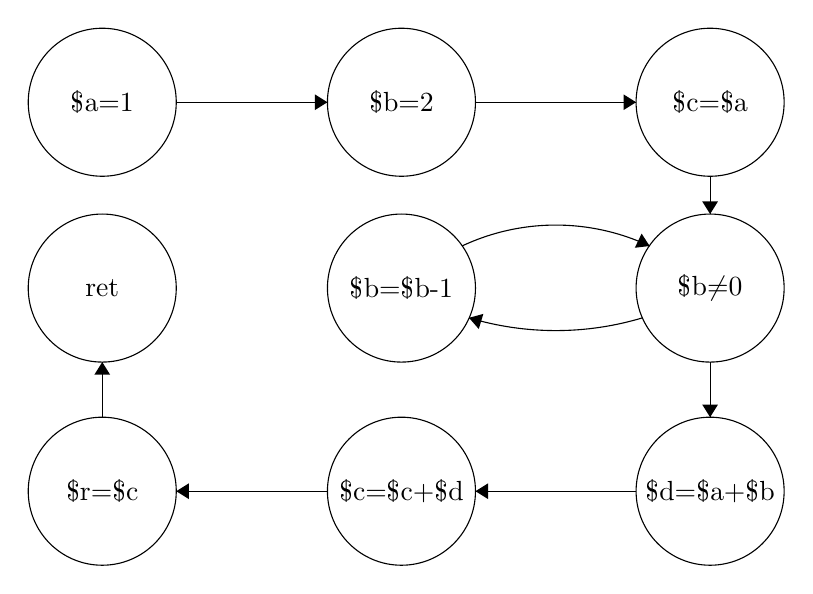
\begin{tikzpicture}[scale=0.2]
            \tikzstyle{every node}+=[inner sep=0pt]
            \draw [black] (11.2,-4.9) circle (4.7);
            \draw (11.2,-4.9) node {\$a=1};
            \draw [black] (30.2,-4.9) circle (4.7);
            \draw (30.2,-4.9) node {\$b=2};
            \draw [black] (49.8,-4.9) circle (4.7);
            \draw (49.8,-4.9) node {\$c=\$a};
            \draw [black] (49.8,-16.7) circle (4.7);
            \draw (49.8,-16.7) node {\$b$\ne$0};
            \draw [black] (30.2,-16.7) circle (4.7);
            \draw (30.2,-16.7) node {\$b=\$b-1};
            \draw [black] (49.8,-29.6) circle (4.7);
            \draw (49.8,-29.6) node {\$d=\$a+\$b};
            \draw [black] (30.2,-29.6) circle (4.7);
            \draw (30.2,-29.6) node {\$c=\$c+\$d};
            \draw [black] (11.2,-16.7) circle (4.7);
            \draw (11.2,-16.7) node {ret};
            \draw [black] (11.2,-29.6) circle (4.7);
            \draw (11.2,-29.6) node {\$r=\$c};
            \draw [black] (15.9,-4.9) -- (25.5,-4.9);
            \fill [black] (25.5,-4.9) -- (24.7,-4.4) -- (24.7,-5.4);
            \draw [black] (34.9,-4.9) -- (45.1,-4.9);
            \fill [black] (45.1,-4.9) -- (44.3,-4.4) -- (44.3,-5.4);
            \draw [black] (49.8,-9.6) -- (49.8,-12);
            \fill [black] (49.8,-12) -- (50.3,-11.2) -- (49.3,-11.2);
            \draw [black] (45.51,-18.59) arc (-73.26619:-106.73381:19.135);
            \fill [black] (34.49,-18.59) -- (35.11,-19.3) -- (35.4,-18.34);
            \draw [black] (34.042,-14.03) arc (115.18117:64.81883:14.004);
            \fill [black] (45.96,-14.03) -- (45.45,-13.24) -- (45.02,-14.14);
            \draw [black] (49.8,-21.4) -- (49.8,-24.9);
            \fill [black] (49.8,-24.9) -- (50.3,-24.1) -- (49.3,-24.1);
            \draw [black] (45.1,-29.6) -- (34.9,-29.6);
            \fill [black] (34.9,-29.6) -- (35.7,-30.1) -- (35.7,-29.1);
            \draw [black] (25.5,-29.6) -- (15.9,-29.6);
            \fill [black] (15.9,-29.6) -- (16.7,-30.1) -- (16.7,-29.1);
            \draw [black] (11.2,-24.9) -- (11.2,-21.4);
            \fill [black] (11.2,-21.4) -- (10.7,-22.2) -- (11.7,-22.2);
        \end{tikzpicture}
    \end{center}
\end{frame}

\begin{frame}{Liveness Analysis}
    \begin{itemize}
        \item To determine the liveness of a variable, from its last use run a (backwards) depth first search
        \item If a node defines the variable, stop searching from that node, but continue searching other paths per depth first search
        \item The edges traversed are where the variable is live
        \pause
        \item Again: two variables can be assigned to the same register if they are not live at the same point in time
        \item We construct an interference graph from the liveness data: two variables have an edge between them if they are live at the same time
    \end{itemize}
\end{frame}

\begin{frame}{Interference Graph of the Code Example}
    \begin{columns}
        \begin{column}{3cm}
            \begin{algo}
                \textul{\textbf{\textsc{Func}}}:\+
                \\ \$a = 1;
                \\ \$b = 2;
                \\ \$c = \$a;
                \\
                \\ \textbf{while} \$b $\ne$ 0 \{\+
                \\ \$b = \$b - 1;\-
                \\ \}
                \\
                \\ \$d = \$a + \$b;
                \\ \$c = \$c + \$d;
                \\
                \\ \$r = \$c;
                \\ \textbf{ret};
            \end{algo}
        \end{column}
        \begin{column}{7cm}
            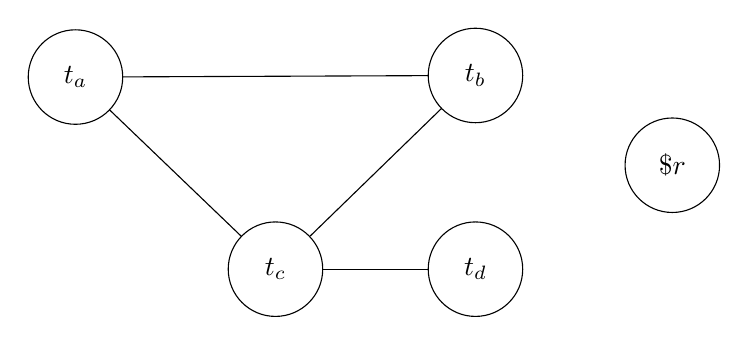
\begin{tikzpicture}[scale=0.2]
                \tikzstyle{every node}+=[inner sep=0pt]
                \draw [black] (3.2,-3.3) circle (3);
                \draw (3.2,-3.3) node {$t_a$};
                \draw [black] (28.6,-3.2) circle (3);
                \draw (28.6,-3.2) node {$t_b$};
                \draw [black] (15.9,-15.5) circle (3);
                \draw (15.9,-15.5) node {$t_c$};
                \draw [black] (28.6,-15.5) circle (3);
                \draw (28.6,-15.5) node {$t_d$};
                \draw [black] (41.1,-8.9) circle (3);
                \draw (41.1,-8.9) node {$\$r$};
                \draw [black] (6.2,-3.29) -- (25.6,-3.21);
                \draw [black] (5.36,-5.38) -- (13.74,-13.42);
                \draw [black] (18.1,-13.4) -- (26.45,-5.29);
                \draw [black] (18.9,-15.5) -- (25.6,-15.5);
            \end{tikzpicture}
        \end{column}
    \end{columns}
\end{frame}

\begin{frame}{Dataflow Analysis in Compilers}
    \begin{itemize}
        \item Liveness analysis is a form of dataflow anaylsis
        \item Dataflow analyses are used everywhere in compiler optimizations
        \pause
        \begin{itemize}
            \item Figure out if one program statement affects a later program statement
            \item Detect and eliminate dead code
            \item Constant and copy propagation
        \end{itemize}
    \end{itemize}
\end{frame}

\begin{frame}{}
      \begin{center}
    {\color{sigma@mainblue} \LARGE Questions?}
  \end{center}
\end{frame}

\section{Graph Coloring Algorithms}
\frame{\sectionpage}

\begin{frame}{Where we are for Register Allocation}
    \begin{itemize}
        \item We have an interference graph representing relationships between variables
        \pause
        \item We can allocate registers by "coloring" variables with a specific register out of $k$ registers total
        \item Register allocation is \textit{nearly} equivalent to graph coloring except that we need store some variables in main memory
        \pause
        \item But graph coloring is NP-Complete
        \begin{itemize}
            \item Imagine that adding one variable to your code doubles the compilation time
            \pause
            \item \textbf{Optimal} graph coloring is NP-Complete
            \item Let's devise an incorrect graph coloring algorithm that is optimal for some but not all cases
        \end{itemize}
    \end{itemize}
\end{frame}

\begin{frame}{Graph Coloring Approximation: Selection}
    \begin{itemize}
        \item Given a graph we want to $k$-color, which vertices can we always assign a color to?
        \pause
        \item Any vertex with less than $k$ neighbors
        \begin{itemize}
            \item Then this vertex is neighboring less than $k$ colors
        \end{itemize}
        \pause
        \item Idea: we can remove vertices with less than $K$ neighbors, add them to a stack, and repeat the process on the reduced graph
        \item We call this the selection phase
        \pause
        \item Some vertices (known registers) start with their corresponding color and are not involved in selection
    \end{itemize}
\end{frame}

\begin{frame}{Selection Example}
    \begin{columns}
        \begin{column}{1cm}
            % \textbf{Stack:}
            % \vspace{0cm}
            
            % $\begin{bmatrix}
            %     \\ \\ \\
            % \end{bmatrix}$
        \end{column}
        \begin{column}{8cm}
            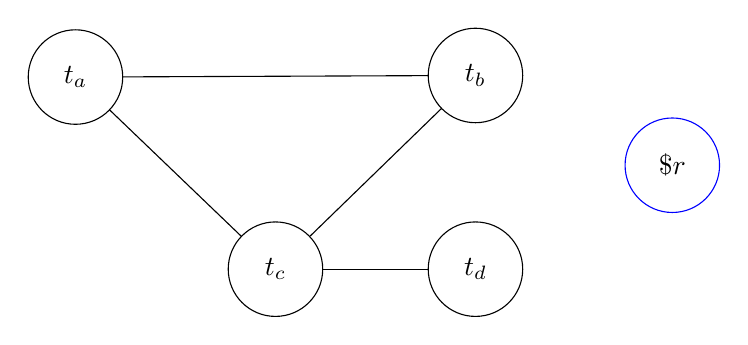
\begin{tikzpicture}[scale=0.2]
            \tikzstyle{every node}+=[inner sep=0pt]
                \draw [black] (3.2,-3.3) circle (3);
                \draw (3.2,-3.3) node {$t_a$};
                \draw [black] (28.6,-3.2) circle (3);
                \draw (28.6,-3.2) node {$t_b$};
                \draw [black] (15.9,-15.5) circle (3);
                \draw (15.9,-15.5) node {$t_c$};
                \draw [black] (28.6,-15.5) circle (3);
                \draw (28.6,-15.5) node {$t_d$};
                \draw [blue] (41.1,-8.9) circle (3);
                \draw (41.1,-8.9) node {$\$r$};
                \draw [black] (6.2,-3.29) -- (25.6,-3.21);
                \draw [black] (5.36,-5.38) -- (13.74,-13.42);
                \draw [black] (18.1,-13.4) -- (26.45,-5.29);
                \draw [black] (18.9,-15.5) -- (25.6,-15.5);
            \end{tikzpicture}
        \end{column}
    \end{columns}
\end{frame}

\begin{frame}{Selection Example}
    \begin{columns}
        \begin{column}{1cm}
            \textbf{Stack:}
            \vspace{0cm}
            
            $\begin{bmatrix}
                \\ \\ \\ t_d
            \end{bmatrix}$
        \end{column}
        \begin{column}{8cm}
            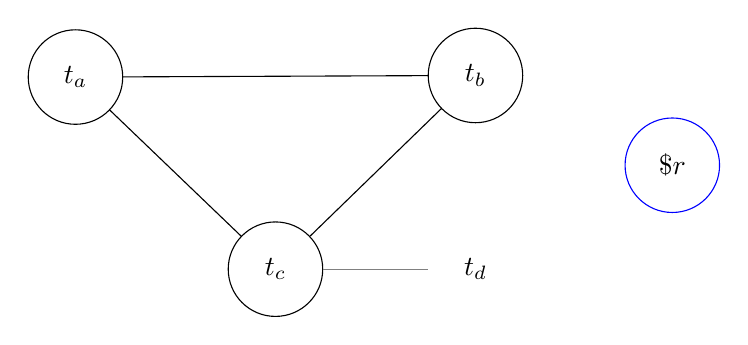
\begin{tikzpicture}[scale=0.2]
            \tikzstyle{every node}+=[inner sep=0pt]
                \draw [black] (3.2,-3.3) circle (3);
                \draw (3.2,-3.3) node {$t_a$};
                \draw [black] (28.6,-3.2) circle (3);
                \draw (28.6,-3.2) node {$t_b$};
                \draw [black] (15.9,-15.5) circle (3);
                \draw (15.9,-15.5) node {$t_c$};
                % \draw [black] (28.6,-15.5) circle (3);
                \draw (28.6,-15.5) node {$t_d$};
                \draw [blue] (41.1,-8.9) circle (3);
                \draw (41.1,-8.9) node {$\$r$};
                \draw [black] (6.2,-3.29) -- (25.6,-3.21);
                \draw [black] (5.36,-5.38) -- (13.74,-13.42);
                \draw [black] (18.1,-13.4) -- (26.45,-5.29);
                \draw [gray] (18.9,-15.5) -- (25.6,-15.5);
            \end{tikzpicture}
        \end{column}
    \end{columns}
\end{frame}

\begin{frame}{Graph Coloring Approximation: Spilling}
    \begin{itemize}
        \item What if we end up with a graph where all vertices have at least $k$ neighbors?
        \begin{itemize}
            \item Can the graph be $k$-colorable?
            \item If not, can we salvage the graph and $k$-color most of the vertices?
        \end{itemize}
        \pause
        \item Pick an arbitrary vertex. Mark it as "spillable," remove it from the graph, add it to the stack, then try to simplify further
        \begin{itemize}
            \item "Spillable" means it may "spill" into main memory
        \end{itemize}
    \end{itemize}
\end{frame}

\begin{frame}{Spilling Example}
    \begin{columns}
        \begin{column}{1cm}
            \textbf{Stack:}
            \vspace{0cm}
            
            $\begin{bmatrix}
                \\ \\ \color{sigma@alertred}{t_c} \\ t_d
            \end{bmatrix}$
        \end{column}
        \begin{column}{8cm}
            \begin{tikzpicture}[scale=0.2]
            \tikzstyle{every node}+=[inner sep=0pt]
                \draw [black] (3.2,-3.3) circle (3);
                \draw (3.2,-3.3) node {$t_a$};
                \draw [black] (28.6,-3.2) circle (3);
                \draw (28.6,-3.2) node {$t_b$};
                % \draw [black] (15.9,-15.5) circle (3);
                \draw (15.9,-15.5) node {$t_c$};
                % \draw [black] (28.6,-15.5) circle (3);
                \draw (28.6,-15.5) node {$t_d$};
                \draw [blue] (41.1,-8.9) circle (3);
                \draw (41.1,-8.9) node {$\$r$};
                \draw [black] (6.2,-3.29) -- (25.6,-3.21);
                \draw [gray] (5.36,-5.38) -- (13.74,-13.42);
                \draw [gray] (18.1,-13.4) -- (26.45,-5.29);
                \draw [gray] (18.9,-15.5) -- (25.6,-15.5);
            \end{tikzpicture}
        \end{column}
    \end{columns}
\end{frame}

\begin{frame}{Spilling Example}
    \begin{columns}
        \begin{column}{1cm}
            \textbf{Stack:}
            \vspace{0cm}
            
            $\begin{bmatrix}
                \\ t_b \\ \color{sigma@alertred}{t_c} \\ t_d
            \end{bmatrix}$
        \end{column}
        \begin{column}{8cm}
            \begin{tikzpicture}[scale=0.2]
            \tikzstyle{every node}+=[inner sep=0pt]
                \draw [black] (3.2,-3.3) circle (3);
                \draw (3.2,-3.3) node {$t_a$};
                % \draw [black] (28.6,-3.2) circle (3);
                \draw (28.6,-3.2) node {$t_b$};
                % \draw [black] (15.9,-15.5) circle (3);
                \draw (15.9,-15.5) node {$t_c$};
                % \draw [black] (28.6,-15.5) circle (3);
                \draw (28.6,-15.5) node {$t_d$};
                \draw [blue] (41.1,-8.9) circle (3);
                \draw (41.1,-8.9) node {$\$r$};
                \draw [gray] (6.2,-3.29) -- (25.6,-3.21);
                \draw [gray] (5.36,-5.38) -- (13.74,-13.42);
                \draw [gray] (18.1,-13.4) -- (26.45,-5.29);
                \draw [gray] (18.9,-15.5) -- (25.6,-15.5);
            \end{tikzpicture}
        \end{column}
    \end{columns}
\end{frame}

\begin{frame}{Spilling Example}
    \begin{columns}
        \begin{column}{1cm}
            \textbf{Stack:}
            \vspace{0cm}
            
            $\begin{bmatrix}
                t_a \\ t_b \\ \color{sigma@alertred}{t_c} \\ t_d
            \end{bmatrix}$
        \end{column}
        \begin{column}{8cm}
            \begin{tikzpicture}[scale=0.2]
            \tikzstyle{every node}+=[inner sep=0pt]
                % \draw [black] (3.2,-3.3) circle (3);
                \draw (3.2,-3.3) node {$t_a$};
                % \draw [black] (28.6,-3.2) circle (3);
                \draw (28.6,-3.2) node {$t_b$};
                % \draw [black] (15.9,-15.5) circle (3);
                \draw (15.9,-15.5) node {$t_c$};
                % \draw [black] (28.6,-15.5) circle (3);
                \draw (28.6,-15.5) node {$t_d$};
                \draw [blue] (41.1,-8.9) circle (3);
                \draw (41.1,-8.9) node {$\$r$};
                \draw [gray] (6.2,-3.29) -- (25.6,-3.21);
                \draw [gray] (5.36,-5.38) -- (13.74,-13.42);
                \draw [gray] (18.1,-13.4) -- (26.45,-5.29);
                \draw [gray] (18.9,-15.5) -- (25.6,-15.5);
            \end{tikzpicture}
        \end{column}
    \end{columns}
\end{frame}

\begin{frame}{Graph Coloring Approximation: Selection}
    \begin{itemize}
        \item Now we have a stack of vertices, some of which may potentially spill (had $\ge k$ neighbors when we removed them)
        \item Let's reconstruct the original graph, but now with color!
        \item There are three cases per vertex we try to re-add to the graph
    \end{itemize}
\end{frame}

\begin{frame}{Graph Coloring Approximation: Selection Cases}
    Vertex was not marked as "spillable"
    \begin{itemize}
        \item Then we know there is a valid color we can assign it; add it back to the graph and color it
    \end{itemize}
\end{frame}

\begin{frame}{Selection Case 1}
    \begin{columns}
        \begin{column}{1cm}
            \textbf{Stack:}
            \vspace{0cm}
            
            $\begin{bmatrix}
                \\ t_b \\ \color{sigma@alertred}{t_c} \\ t_d
            \end{bmatrix}$
        \end{column}
        \begin{column}{8cm}
            \begin{tikzpicture}[scale=0.2]
            \tikzstyle{every node}+=[inner sep=0pt]
                \draw [blue] (3.2,-3.3) circle (3);
                \draw (3.2,-3.3) node {$t_a$};
                % \draw [black] (28.6,-3.2) circle (3);
                \draw (28.6,-3.2) node {$t_b$};
                % \draw [black] (15.9,-15.5) circle (3);
                \draw (15.9,-15.5) node {$t_c$};
                % \draw [black] (28.6,-15.5) circle (3);
                \draw (28.6,-15.5) node {$t_d$};
                \draw [blue] (41.1,-8.9) circle (3);
                \draw (41.1,-8.9) node {$\$r$};
                \draw [gray] (6.2,-3.29) -- (25.6,-3.21);
                \draw [gray] (5.36,-5.38) -- (13.74,-13.42);
                \draw [gray] (18.1,-13.4) -- (26.45,-5.29);
                \draw [gray] (18.9,-15.5) -- (25.6,-15.5);
            \end{tikzpicture}
        \end{column}
    \end{columns}
\end{frame}

\begin{frame}{Selection Case 1}
    \begin{columns}
        \begin{column}{1cm}
            \textbf{Stack:}
            \vspace{0cm}
            
            $\begin{bmatrix}
                \\ \\ \color{sigma@alertred}{t_c} \\ t_d
            \end{bmatrix}$
        \end{column}
        \begin{column}{8cm}
            \begin{tikzpicture}[scale=0.2]
            \tikzstyle{every node}+=[inner sep=0pt]
                \draw [blue] (3.2,-3.3) circle (3);
                \draw (3.2,-3.3) node {$t_a$};
                \draw [green] (28.6,-3.2) circle (3);
                \draw (28.6,-3.2) node {$t_b$};
                % \draw [black] (15.9,-15.5) circle (3);
                \draw (15.9,-15.5) node {$t_c$};
                % \draw [black] (28.6,-15.5) circle (3);
                \draw (28.6,-15.5) node {$t_d$};
                \draw [blue] (41.1,-8.9) circle (3);
                \draw (41.1,-8.9) node {$\$r$};
                \draw [black] (6.2,-3.29) -- (25.6,-3.21);
                \draw [gray] (5.36,-5.38) -- (13.74,-13.42);
                \draw [gray] (18.1,-13.4) -- (26.45,-5.29);
                \draw [gray] (18.9,-15.5) -- (25.6,-15.5);
            \end{tikzpicture}
        \end{column}
    \end{columns}
\end{frame}

\begin{frame}{Graph Coloring Approximation: Selection Cases (Continued)}
    Vertex was marked as "spillable" but has a valid coloring
    \begin{itemize}
        \item Then re-add the vertex and assign it a valid color
        \item This will not impact other vertices not marked as "spillable"
    \end{itemize}
\end{frame}

\begin{frame}{Graph Coloring Approximation: Selection Cases (Continued)}
    \begin{itemize}
        \item Vertex was marked as "spillable" and does not have a valid coloring
        \begin{itemize}
            \item We will generate instructions to store/fetch this variable to/from main memory
        \end{itemize}
    \end{itemize}
\end{frame}

\begin{frame}{Selection Cases 2 and 3}
    \begin{columns}
        \begin{column}{1cm}
            \textbf{Stack:}
            \vspace{0cm}
            
            $\begin{bmatrix}
                \\ \\ \\ t_d
            \end{bmatrix}$
        \end{column}
        \begin{column}{8cm}
            \begin{tikzpicture}[scale=0.2]
            \tikzstyle{every node}+=[inner sep=0pt]
                \draw [blue] (3.2,-3.3) circle (3);
                \draw (3.2,-3.3) node {$t_a$};
                \draw [green] (28.6,-3.2) circle (3);
                \draw (28.6,-3.2) node {$t_b$};
                \draw [red] (15.9,-15.5) circle (3);
                \draw (15.9,-15.5) node {\color{sigma@alertred}{$t_c$}};
                % \draw [black] (28.6,-15.5) circle (3);
                \draw (28.6,-15.5) node {$t_d$};
                \draw [blue] (41.1,-8.9) circle (3);
                \draw (41.1,-8.9) node {$\$r$};
                \draw [black] (6.2,-3.29) -- (25.6,-3.21);
                \draw [black] (5.36,-5.38) -- (13.74,-13.42);
                \draw [black] (18.1,-13.4) -- (26.45,-5.29);
                \draw [gray] (18.9,-15.5) -- (25.6,-15.5);
            \end{tikzpicture}
        \end{column}
    \end{columns}
\end{frame}

\begin{frame}{Graph Coloring Approximation: Spilled Nodes}
    \begin{itemize}
        \item Can we continue running the algorithm?
        \pause
        \item No! The instructions to store/fetch the node to/from main memory use temporary variables
        \item We rebuild the interference graph and rerun the graph coloring algorithm
        \pause
        \item Problem: we introduced new temporary variables, what if the new graph can't be colored?
        \pause
        \item The new temporary variables have a very short time they are live; we will eventually converge on a $k$-coloring with spilling
    \end{itemize}
\end{frame}

\begin{frame}{}
      \begin{center}
    {\color{sigma@mainblue} \LARGE Questions?}
  \end{center}
\end{frame}

\begin{frame}{Graph Coloring Approximation Optimality}
    \begin{itemize}
        \item This algorithm takes $O(n)$ time in the best case, $O(n^2)$ time in the worst case
        \item This graph coloring algorithm seems to work well, but is \textbf{not} optimal
    \end{itemize}
\end{frame}

\begin{frame}{Optimality Counter Example}
    \begin{columns}
        \begin{column}{1cm}
            % \textbf{Stack:}
            % \vspace{0cm}
            
            % $\begin{bmatrix}
            %     \\ \\ \\ \\ \\
            % \end{bmatrix}$
        \end{column}
        \begin{column}{8cm}
            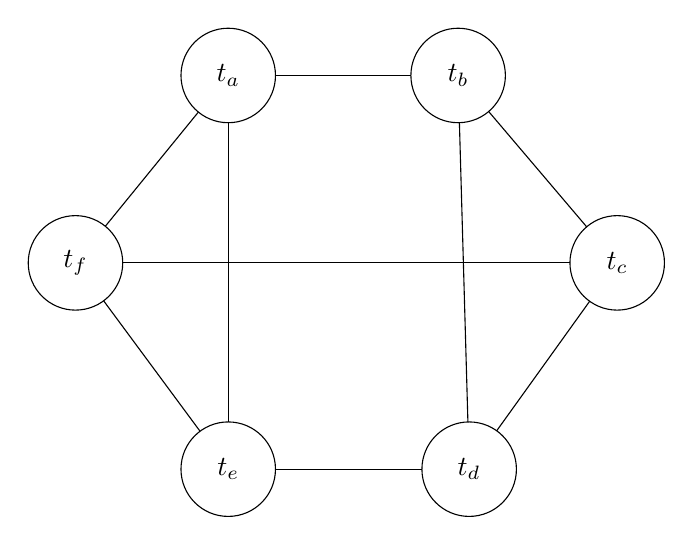
\begin{tikzpicture}[scale=0.2]
                \tikzstyle{every node}+=[inner sep=0pt]
                \draw [black] (27.5,-3.2) circle (3);
                \draw (27.5,-3.2) node {$t_b$};
                \draw [black] (37.6,-15.1) circle (3);
                \draw (37.6,-15.1) node {$t_c$};
                \draw [black] (3.2,-15.1) circle (3);
                \draw (3.2,-15.1) node {$t_f$};
                \draw [black] (12.9,-28.2) circle (3);
                \draw (12.9,-28.2) node {$t_e$};
                \draw [black] (28.2,-28.2) circle (3);
                \draw (28.2,-28.2) node {$t_d$};
                \draw [black] (12.9,-3.2) circle (3);
                \draw (12.9,-3.2) node {$t_a$};
                \draw [black] (29.44,-5.49) -- (35.66,-12.81);
                \draw [black] (27.58,-6.2) -- (28.12,-25.2);
                \draw [black] (35.85,-17.54) -- (29.95,-25.76);
                \draw [black] (25.2,-28.2) -- (15.9,-28.2);
                \draw [black] (11.11,-25.79) -- (4.99,-17.51);
                \draw [black] (24.5,-3.2) -- (15.9,-3.2);
                \draw [black] (11,-5.53) -- (5.1,-12.77);
                \draw [black] (12.9,-6.2) -- (12.9,-25.2);
                \draw [black] (6.2,-15.1) -- (34.6,-15.1);
            \end{tikzpicture}
        \end{column}
    \end{columns}
\end{frame}

\begin{frame}{Optimality Counter Example}
    \begin{columns}
        \begin{column}{1cm}
            \textbf{Stack:}
            \vspace{0cm}
            
            $\begin{bmatrix}
                \\ \\ \\ \\ \\ t_c
            \end{bmatrix}$
        \end{column}
        \begin{column}{8cm}
            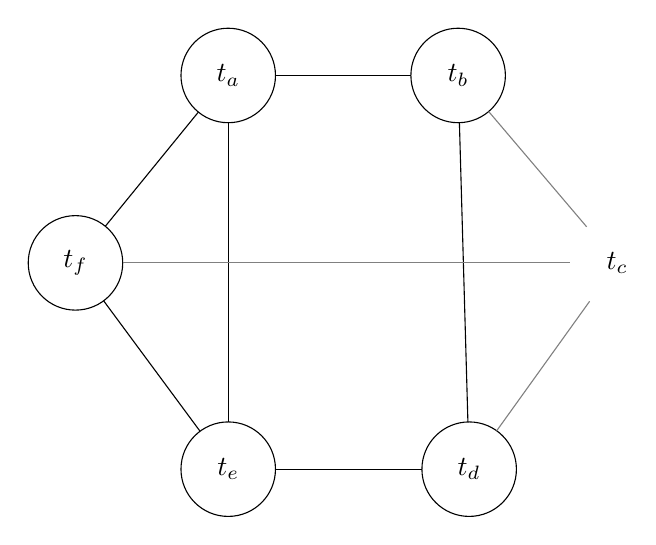
\begin{tikzpicture}[scale=0.2]
                \tikzstyle{every node}+=[inner sep=0pt]
                \draw [black] (27.5,-3.2) circle (3);
                \draw (27.5,-3.2) node {$t_b$};
                % \draw [black] (37.6,-15.1) circle (3);
                \draw (37.6,-15.1) node {$t_c$};
                \draw [black] (3.2,-15.1) circle (3);
                \draw (3.2,-15.1) node {$t_f$};
                \draw [black] (12.9,-28.2) circle (3);
                \draw (12.9,-28.2) node {$t_e$};
                \draw [black] (28.2,-28.2) circle (3);
                \draw (28.2,-28.2) node {$t_d$};
                \draw [black] (12.9,-3.2) circle (3);
                \draw (12.9,-3.2) node {$t_a$};
                \draw [gray] (29.44,-5.49) -- (35.66,-12.81);
                \draw [black] (27.58,-6.2) -- (28.12,-25.2);
                \draw [gray] (35.85,-17.54) -- (29.95,-25.76);
                \draw [black] (25.2,-28.2) -- (15.9,-28.2);
                \draw [black] (11.11,-25.79) -- (4.99,-17.51);
                \draw [black] (24.5,-3.2) -- (15.9,-3.2);
                \draw [black] (11,-5.53) -- (5.1,-12.77);
                \draw [black] (12.9,-6.2) -- (12.9,-25.2);
                \draw [gray] (6.2,-15.1) -- (34.6,-15.1);
            \end{tikzpicture}
        \end{column}
    \end{columns}
\end{frame}

\begin{frame}{Optimality Counter Example}
    \begin{columns}
        \begin{column}{1cm}
            \textbf{Stack:}
            \vspace{0cm}
            
            $\begin{bmatrix}
                t_f \\ t_e \\ t_a \\ t_d \\ t_b \\ t_c
            \end{bmatrix}$
        \end{column}
        \begin{column}{8cm}
            \begin{tikzpicture}[scale=0.2]
                \tikzstyle{every node}+=[inner sep=0pt]
                % \draw [black] (27.5,-3.2) circle (3);
                \draw (27.5,-3.2) node {$t_b$};
                % \draw [black] (37.6,-15.1) circle (3);
                \draw (37.6,-15.1) node {$t_c$};
                % \draw [black] (3.2,-15.1) circle (3);
                \draw (3.2,-15.1) node {$t_f$};
                % \draw [black] (12.9,-28.2) circle (3);
                \draw (12.9,-28.2) node {$t_e$};
                % \draw [black] (28.2,-28.2) circle (3);
                \draw (28.2,-28.2) node {$t_d$};
                % \draw [black] (12.9,-3.2) circle (3);
                \draw (12.9,-3.2) node {$t_a$};
                \draw [gray] (29.44,-5.49) -- (35.66,-12.81);
                \draw [gray] (27.58,-6.2) -- (28.12,-25.2);
                \draw [gray] (35.85,-17.54) -- (29.95,-25.76);
                \draw [gray] (25.2,-28.2) -- (15.9,-28.2);
                \draw [gray] (11.11,-25.79) -- (4.99,-17.51);
                \draw [gray] (24.5,-3.2) -- (15.9,-3.2);
                \draw [gray] (11,-5.53) -- (5.1,-12.77);
                \draw [gray] (12.9,-6.2) -- (12.9,-25.2);
                \draw [gray] (6.2,-15.1) -- (34.6,-15.1);
            \end{tikzpicture}
        \end{column}
    \end{columns}
\end{frame}

\begin{frame}{Optimality Counter Example}
    \begin{columns}
        \begin{column}{1cm}
            \textbf{Stack:}
            \vspace{0cm}
            
            $\begin{bmatrix}
                \\ \\ \\ t_d \\ t_b \\ t_c
            \end{bmatrix}$
        \end{column}
        \begin{column}{8cm}
            \begin{tikzpicture}[scale=0.2]
                \tikzstyle{every node}+=[inner sep=0pt]
                % \draw [black] (27.5,-3.2) circle (3);
                \draw (27.5,-3.2) node {$t_b$};
                % \draw [black] (37.6,-15.1) circle (3);
                \draw (37.6,-15.1) node {$t_c$};
                \draw [blue] (3.2,-15.1) circle (3);
                \draw (3.2,-15.1) node {$t_f$};
                \draw [green] (12.9,-28.2) circle (3);
                \draw (12.9,-28.2) node {$t_e$};
                % \draw [black] (28.2,-28.2) circle (3);
                \draw (28.2,-28.2) node {$t_d$};
                \draw [red] (12.9,-3.2) circle (3);
                \draw (12.9,-3.2) node {$t_a$};
                \draw [gray] (29.44,-5.49) -- (35.66,-12.81);
                \draw [gray] (27.58,-6.2) -- (28.12,-25.2);
                \draw [gray] (35.85,-17.54) -- (29.95,-25.76);
                \draw [gray] (25.2,-28.2) -- (15.9,-28.2);
                \draw [black] (11.11,-25.79) -- (4.99,-17.51);
                \draw [gray] (24.5,-3.2) -- (15.9,-3.2);
                \draw [black] (11,-5.53) -- (5.1,-12.77);
                \draw [black] (12.9,-6.2) -- (12.9,-25.2);
                \draw [gray] (6.2,-15.1) -- (34.6,-15.1);
            \end{tikzpicture}
        \end{column}
    \end{columns}
\end{frame}

\begin{frame}{Optimality Counter Example}
    \begin{columns}
        \begin{column}{1cm}
            \textbf{Stack:}
            \vspace{0cm}
            
            $\begin{bmatrix}
                \\ \\ \\ \\ \\ t_c
            \end{bmatrix}$
        \end{column}
        \begin{column}{8cm}
            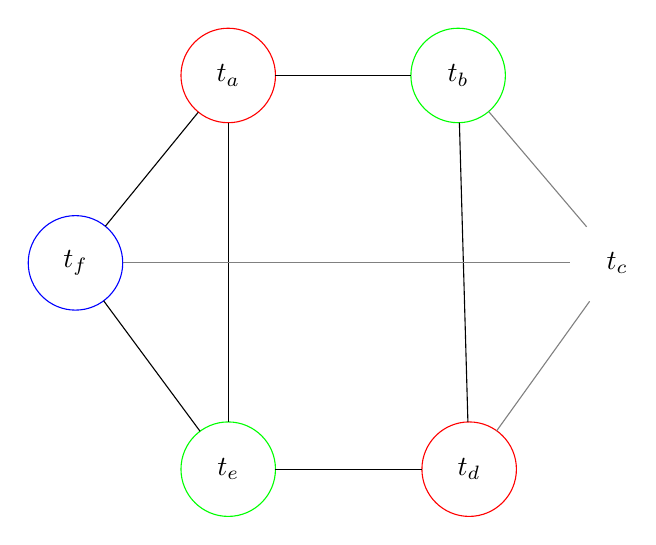
\begin{tikzpicture}[scale=0.2]
                \tikzstyle{every node}+=[inner sep=0pt]
                \draw [green] (27.5,-3.2) circle (3);
                \draw (27.5,-3.2) node {$t_b$};
                % \draw [black] (37.6,-15.1) circle (3);
                \draw (37.6,-15.1) node {$t_c$};
                \draw [blue] (3.2,-15.1) circle (3);
                \draw (3.2,-15.1) node {$t_f$};
                \draw [green] (12.9,-28.2) circle (3);
                \draw (12.9,-28.2) node {$t_e$};
                \draw [red] (28.2,-28.2) circle (3);
                \draw (28.2,-28.2) node {$t_d$};
                \draw [red] (12.9,-3.2) circle (3);
                \draw (12.9,-3.2) node {$t_a$};
                \draw [gray] (29.44,-5.49) -- (35.66,-12.81);
                \draw [black] (27.58,-6.2) -- (28.12,-25.2);
                \draw [gray] (35.85,-17.54) -- (29.95,-25.76);
                \draw [black] (25.2,-28.2) -- (15.9,-28.2);
                \draw [black] (11.11,-25.79) -- (4.99,-17.51);
                \draw [black] (24.5,-3.2) -- (15.9,-3.2);
                \draw [black] (11,-5.53) -- (5.1,-12.77);
                \draw [black] (12.9,-6.2) -- (12.9,-25.2);
                \draw [gray] (6.2,-15.1) -- (34.6,-15.1);
            \end{tikzpicture}
        \end{column}
    \end{columns}
\end{frame}

\begin{frame}{Optimality Counter Example}
    \begin{columns}
        \begin{column}{1cm}
            % \textbf{Stack:}
            % \vspace{0cm}
            
            % $\begin{bmatrix}
            %     \\ \\ \\ \\ \\
            % \end{bmatrix}$
        \end{column}
        \begin{column}{8cm}
            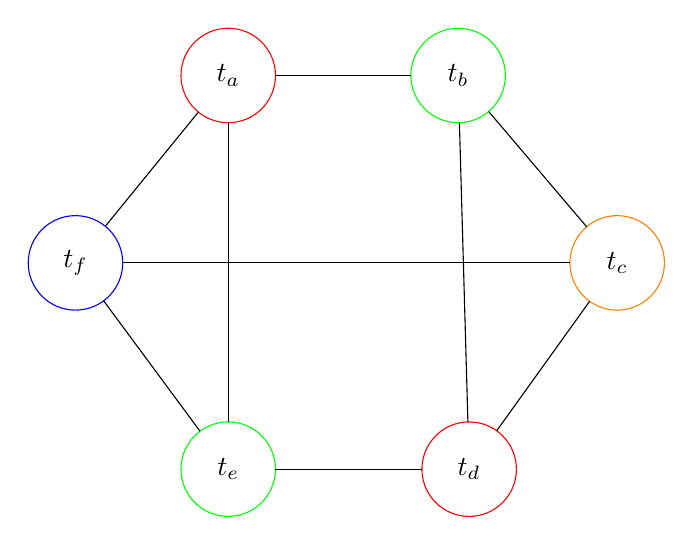
\begin{tikzpicture}[scale=0.2]
                \tikzstyle{every node}+=[inner sep=0pt]
                \draw [green] (27.5,-3.2) circle (3);
                \draw (27.5,-3.2) node {$t_b$};
                \draw [orange] (37.6,-15.1) circle (3);
                \draw (37.6,-15.1) node {$t_c$};
                \draw [blue] (3.2,-15.1) circle (3);
                \draw (3.2,-15.1) node {$t_f$};
                \draw [green] (12.9,-28.2) circle (3);
                \draw (12.9,-28.2) node {$t_e$};
                \draw [red] (28.2,-28.2) circle (3);
                \draw (28.2,-28.2) node {$t_d$};
                \draw [red] (12.9,-3.2) circle (3);
                \draw (12.9,-3.2) node {$t_a$};
                \draw [black] (29.44,-5.49) -- (35.66,-12.81);
                \draw [black] (27.58,-6.2) -- (28.12,-25.2);
                \draw [black] (35.85,-17.54) -- (29.95,-25.76);
                \draw [black] (25.2,-28.2) -- (15.9,-28.2);
                \draw [black] (11.11,-25.79) -- (4.99,-17.51);
                \draw [black] (24.5,-3.2) -- (15.9,-3.2);
                \draw [black] (11,-5.53) -- (5.1,-12.77);
                \draw [black] (12.9,-6.2) -- (12.9,-25.2);
                \draw [black] (6.2,-15.1) -- (34.6,-15.1);
            \end{tikzpicture}
        \end{column}
    \end{columns}
\end{frame}

\begin{frame}{Optimal Solution}
    \begin{columns}
        \begin{column}{1cm}
            % \textbf{Stack:}
            % \vspace{0cm}
            
            % $\begin{bmatrix}
            %     \\ \\ \\ \\ \\
            % \end{bmatrix}$
        \end{column}
        \begin{column}{8cm}
            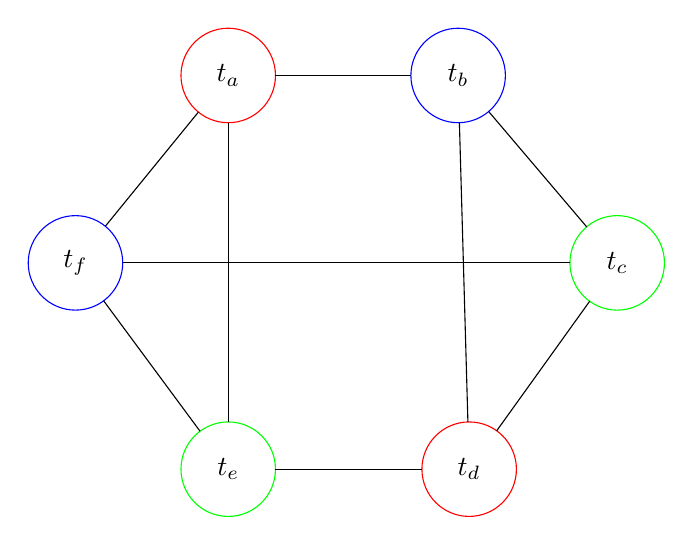
\begin{tikzpicture}[scale=0.2]
                \tikzstyle{every node}+=[inner sep=0pt]
                \draw [blue] (27.5,-3.2) circle (3);
                \draw (27.5,-3.2) node {$t_b$};
                \draw [green] (37.6,-15.1) circle (3);
                \draw (37.6,-15.1) node {$t_c$};
                \draw [blue] (3.2,-15.1) circle (3);
                \draw (3.2,-15.1) node {$t_f$};
                \draw [green] (12.9,-28.2) circle (3);
                \draw (12.9,-28.2) node {$t_e$};
                \draw [red] (28.2,-28.2) circle (3);
                \draw (28.2,-28.2) node {$t_d$};
                \draw [red] (12.9,-3.2) circle (3);
                \draw (12.9,-3.2) node {$t_a$};
                \draw [black] (29.44,-5.49) -- (35.66,-12.81);
                \draw [black] (27.58,-6.2) -- (28.12,-25.2);
                \draw [black] (35.85,-17.54) -- (29.95,-25.76);
                \draw [black] (25.2,-28.2) -- (15.9,-28.2);
                \draw [black] (11.11,-25.79) -- (4.99,-17.51);
                \draw [black] (24.5,-3.2) -- (15.9,-3.2);
                \draw [black] (11,-5.53) -- (5.1,-12.77);
                \draw [black] (12.9,-6.2) -- (12.9,-25.2);
                \draw [black] (6.2,-15.1) -- (34.6,-15.1);
            \end{tikzpicture}
        \end{column}
    \end{columns}
\end{frame}

\begin{frame}{Register Allocation: Further Optimizations}
    \begin{itemize}
        \item Many instructions of the form of $t_a = t_b$ can be eliminated such that $t_a$ shares the same register or main memory address as $t_b$ -- this is move coalescing
        \pause
        \item Allows us to do this
        \begin{columns}
            \begin{column}{2cm}
                \begin{algo}
                    \textul{\textbf{\textsc{Func}}}:\+
                    \\ \$a = 1;
                    \\ \$b = 2;
                    \\ \vdots
                    \\ \textcolor{sigma@alertred}{\$a} = \textcolor{sigma@alertred}{\$a} + \$b;
                    \\
                    \\ \$r = \textcolor{sigma@alertred}{\$a};
                    \\ \textbf{ret};
                \end{algo}
            \end{column}
            \begin{column}{2cm}
                \begin{algo}
                    \textul{\textbf{\textsc{Func}}}:\+
                    \\ \textcolor{sigma@alertred}{\$r} = 1;
                    \\ \$b = 2;
                    \\ \vdots
                    \\ \textcolor{sigma@alertred}{\$r} = \textcolor{sigma@alertred}{\$r} + \$b;
                    \\
                    \\ \textbf{ret};
                \end{algo}
            \end{column}
        \end{columns}
    \end{itemize}
\end{frame}

\begin{frame}{Register Allocation: Further Optimizations (Continued)}
    \begin{itemize}
        \item We can also enforce more strict rules for creating edges in the interference graph after dataflow analysis
        \item Simplify-Spill-Select turns into Simplify-Coalesce-Freeze-Spill-Select
        \item Many places where we can introduce heuristics into the graph coloring algorithm
        \item If we have to restart the algorithm due to spilling, we can reuse a lot of work
        \pause
        \item Optimal register allocation is possible for expression trees
    \end{itemize}
\end{frame}

\section{Conclusion}
\frame{\sectionpage}

\begin{frame}{Takeaways}
    \begin{itemize}
        \item Graph coloring is an NP-Complete problem
        \item Graph coloring is vitally important to optimizing compilers
        \item Given compilers implement a lot of graph algorithms, if P=NP we could potentially make a lot more optimizations
        \pause
        \item However, heuristic approximations to NP hard graph problems already yield an optimal or close to optimal solution in most cases
    \end{itemize}
\end{frame}

\begin{frame}{}
      \begin{center}
    {\color{sigma@mainblue} \LARGE Questions?}
  \end{center}
\end{frame}

\font\eightss=cmssq8
\font\eightssi=cmssqi8
\newcommand\quoteAuthorDate[3]{\begingroup
  \baselineskip 10pt
  \parfillskip 0pt
  \interlinepenalty 10000 % not needed in example
  \leftskip 0pt plus 40pc minus \parindent
  \let\rm=\eightss
  \let\sl=\eightssi
  \everypar{\sl}#1\par
  \nobreak\smallskip
  \noindent\rm--- #2\unskip\enspace(#3)\par
  \endgroup}
% If someone can figure out how to horizontally center this and make the text bigger that'd be cool
\begin{frame}{Brainteaser}
    \begin{center}
        \item A plane with 100 seats is to be boarded by 100 passengers, each with an assigned seat. The first person to board forgot their assignment, so will choose any seat at random. The remaining passengers all sit in their assigned seat, unless it is taken, in which case they chose one of the remaining seats at random. What is the probability the last passenger will sit in their assigned seat. 
    \end{center}
\end{frame}

% Remove this slide if you came up with all the material yourself
\begin{frame}[allowframebreaks]{Bibliography}
    \tiny
    \bibliography{refs}
    \bibliographystyle{alpha}
    
\end{frame}

\end{document}